\cotefile{70}
\scanpage{2}
$n$-polyêdres et $n$-hyperpolyêdres
% archive sheet number: 1
\scanpage{3}
(23 p)

$n$-\unsure{polyèdres|polyedres} réguliers en \unsure{coordonnées|coordonnees} affines universelles

(vieille rédaction)
% archive sheet number: 2
\scanpage{4}
$n$-polyèdres réguliers.

Considérons \deleted{\unsure{le|la}} une $n$-carte régulière, défini par un espace homogène $\underline{R}$ \inserted{(\unsure{tt plein})} sous le groupe $n$-cartographique
\[
\begin{aligned}
G_n=\{\sigma_0,\ldots,\sigma_n\mid {}&\sigma_0^2=\cdots=\sigma_n^2=1\\
&\sigma_i\sigma_j=\sigma_j\sigma_i\quad\text{si }\left\{\begin{aligned}&\deleted{\unsure{i< i+j}}\inserted{j\geq i+2}\\&0\leq i,j\leq n\end{aligned}\right.\}
\end{aligned}
\]
tel que les stabilisateurs \deleted{de}\inserted{$G_{n\underline{x}}$} $\forall\,\underline{x}\in\underline{R}$ sont distingués dans $G_n$, donc indépendants de $x$, soit $H$, \inserted{et $G_n/H=\Gamma$} On suppose que pour tte partie $\unsure{J|I}$ de $[0,n]\cap\mathbb{N}$ ne contenant pas deux entiers consécutifs, le produit \deleted{de} $\sigma_J=\prod_{i\in J}\sigma_i\notin H$ i.e. le produit $\sigma_H$ des $\sigma_i$ \uline{dans} $\Gamma$ est $\neq1$.
% slanted
\margin{inutile \dots}

On pose
\[
\left\{\begin{aligned}
p_1&=\text{ordre de }\sigma_0\sigma_1\\
&\cdots\\
p_n&=\text{ordre de }\sigma_{n-1}\sigma_n
\end{aligned}\right.
\]
\margin{\uline{NB} les $p_i$ peuvent être infinis !}
et on suppose
\[
3\leq p_i\leq+\infty\qquad\text{pour }1\leq i\leq n
\]
\margin{i)}
On suppose ici que $\Gamma$ est le groupe engendré par les $\sigma_i$, avec (en plus des relations plus haut définissant $G_n$) les relations supplémentaires
\[
(\sigma_{i-1}\sigma_i)^{p_i}=1
\]
% archive sheet number: 3
\scanpage{5}
si
\[
p_*=(p_1,\ldots,p_n)\in([3,+\infty]\cap\overline{\mathbb{N}})^n
\]
\deleted{$\unsure{\underline{R}=\Gamma}$}
\[
\Gamma=\Gamma_{p_*}
\]
est entièrement déterminé par $p_*$ et, quel que soit $p_*$, les conditions \deleted{$\unsure{\sigma_J\neq1|\sigma_I\neq1}\text{ dans }\Gamma_{p_*}$}
\[
\sigma_J\neq1\quad\text{dans }\Gamma_{p_*}
\]
sont satisfaites dans $\Gamma=\Gamma_{p_*}$. Tous les $\underline{R}$ sont isom. entre eux, et quand on prend des $\underline{R}$ munis d'un ``repère'' $\alpha\in R$, ils sont canoniquement isom. entre eux, et \inserted{can.} isom. à \deleted{$\unsure{E|R}$}
\[
\underline{R}_{p_*}=G_n/\Gamma_{p_*}
\]
munis du repère image de $1\in G_n$.

Pour tte partie $H$ de \deleted{$\unsure{G}$} $[0,n]\cap\mathbb{N}$, on désigne par $G_{nH}$ le sous-groupe de $G_n$ engendré par les $\sigma_i$, $i\notin H$. Donc
\[
H\subset K\longrightarrow G_K\subset G_H
\]
\diagram{\begin{tikzcd}[ampersand replacement=\&]
\underline{R}/G_K \arrow[r] \arrow[d,equal] \& \underline{R}/G_H \arrow[d,equal]\\
D_K \& D_H
\end{tikzcd}}
Si $H=\{i\}$, on trouve
\[
\begin{aligned}
D_{\{i\}}=D_i&=\text{ens des }i\text{-facettes}\\
&\text{du }\unsure{p|n}\text{-polyèdre régulier }\Pi\\
&\text{défini par le}
\end{aligned}
\]
% archive sheet number: 4
\scanpage{6}
Sauf erreur, on est dans les conditions qu'il faut pour que la \deleted{polyèdre comb.}\inserted{carte comb.} régulière définie par la $n$-carte $R\simeq R_{p_*}$ soit défini par une \uline{géométrie d'incidence} ayant \deleted{les} $D_i$ comme ens des facettes de dim $i$ (donc soit un polyèdre comb. régulier \inserted{$\Pi$}).

Une \uline{réalisation géom.} \inserted{\uline{affine régulière}} de $\Pi$ \deleted{est} sur un \deleted{schéma} anneau comm. $k$ (disons) est la donnée

a) d'un torseur (espace $k$-affine) \inserted{$E$} sous un $k$-Module loc libre de rang $n+1$

b) d'applications
\[
\begin{aligned}
\unsure{\varphi|\phi}_i:D_i\longrightarrow{}&\text{ens des sous-esp. affines}\\
&\text{de dim }i\text{ dans }E
\end{aligned}
\]
\[
(0\leq i\leq n)
\]
respectant les relations d'incidences,

\deleted{c) d'un hom. de groupes}\inserted{avec condition supplémentaire}

\unsure{par|$\rho$} \deleted{\unsure{par}}
\diagram{\begin{tikzcd}[ampersand replacement=\&]
\deleted{\operatorname{Aut}(\Pi)} \arrow[r,phantom,"\deleted{\longrightarrow}" description] \& \deleted{\operatorname{Autaff}(E)}
\end{tikzcd}}
\deleted{\unsure{tel}} \deleted{compatible avec les}

c)
\[
\left\{\begin{aligned}
&\forall g\in\operatorname{Aut}(\Pi),\quad\exists!\ \bar{g}\in\operatorname{Aff}(E)\quad\text{tel que}\\
&\bar{g}\circ\varphi_i=\varphi_i\circ g_{D_i}\qquad\forall\ 0\leq i\leq n.
\end{aligned}\right.
\]
--- et cette unicité est \unsure{vrai|vraie} fibre par fibre \dots
% archive sheet number: 5
\scanpage{7}
\margin{à vérifier}
Il revient au $=$ de se donner une application
\[
\unsure{\varphi|\phi}_R:\underline{R}\longrightarrow\deleted{\unsure{\operatorname{Repaff}}(E)}\operatorname{Drap.aff}_n(E)
\]
\margin{drapeaux maximaux de $E$}
et \deleted{un homo} et un \deleted{tel qu'il existe un unique} homo
\diagram{\begin{tikzcd}[ampersand replacement=\&]
G \arrow[r,"\varphi_G"] \& \operatorname{Aut}\operatorname{aff}E
\end{tikzcd}}
compatible avec $\varphi_R$, tel que les sommets des \deleted{repères} drapeaux de l'image de $\underline{R}$ engendrent affinement $E$. (ce qui implique l'unicité de $\varphi_G$ \unsure{élément} par \unsure{élément} \dots), et la condition suivante :

\inserted{le sous-groupe $G_{f_i}$ de $G$ stabilisateur de la composante $f_i$ de dim $i$ d'un ``repère'' $\underline{r}\in\underline{R}$, opérant sur $E$, \unsure{invarie} \deleted{la composante} $F_i$ de l'image $r$ de $\underline{r}$ par $\varphi$}
% insertion continues into the left margin, slanted

Comme $\underline{R}$ est un \unsure{torseur|espace} sous $G$, il suffit en fait, étant choisi une origine $\underline{r}\in\underline{R}$, \inserted{permettant d'identifier $\underline{R}\unsure{:|\simeq}R_{p_*}$}, de se donner $\varphi_{G\inserted{=\Gamma}}$ et $\varphi_R(\underline{r})=r\in\operatorname{Drap.aff}_n(E)$, avec comme seules conditions que

a) \deleted{$\unsure{\{}$} Si $j\neq i$, $\sigma_j$ \unsure{invarie} $f_j$

b) les $g.f_0$ ($g\in G=\Gamma$) engendrent \inserted{affinement $E$ fibre par fibre \dots}
% archive sheet number: 6
\scanpage{8}
Posons
\[
\left\{\begin{aligned}
s_0&=f_0\\
s_1&=\sigma_0.f_0\\
s_2&=\sigma_1s_1\\
&\cdots\\
s_i&=\sigma_{i-1}s_{i-1}\\
&\cdots\\
s_{\deleted{\unsure{n}}n+1}&=\sigma_ns_n
\end{aligned}\right.
\]
Je dis que les $(s_i)_{0\leq i\leq n+1}$ \unsure{forment|forme} une \uline{base Affine} de $E$ fibre par fibre, \inserted{et que $f_i=\text{env. aff. de }(s_0\text{--}s_i)$, $0\leq i\leq n$} \deleted{$\unsure{f_i=s_i}$}, et que \inserted{$\sigma_i s_j=s_j$ si $i>j$;} Supposons prouvé, \inserted{pour $i$ donné $0\leq i<n$, que $\{s_0,\ldots,s_j\}$ \unsure{affinemt libre}, $f_j=\text{enveloppe affine de }\{s_0\text{--}s_j\}$, $0\leq j\leq i$,} \deleted{ceci étant trivial pr $i=0$). (Il faut \unsure{prouver}} enfin $\sigma_k s_j=s_j$ si \deleted{$\unsure{j<i}$}\inserted{$k>j$}, \deleted{\unsure{toujours}} pour $j\leq i$. Prouvons que \inserted{fibre par fibre} $s_{i+1}=\sigma_i s_i$ n'appartient pas à \inserted{l'enveloppe} affine $f_i$ de $\{s_0,\ldots,s_i\}$, et \inserted{plus précisément} que $f_{i+1}$ est l'enveloppe affine de $\{s_0,\ldots,s_i,\inserted{s_{i+1}=}\sigma_i s_i\}$, \deleted{\unsure{Et}} puis \inserted{que $\sigma_k s_{i+1}=s_{i+1}$ si $k>i+1$.} \unsure{D'abord|Évident}, comme $s_i\in f_i\subset f_{i+1}$ et $\sigma_i$ fixe $f_{i+1}$, on a $\inserted{s_{i+1}=}\sigma_i(s_i)\in f_{i+1}$, donc il faut seulement prouver que $\sigma_i(s_i)\notin f_i$. \deleted{Mais si}\inserted{\unsure{plus encore que} sur les fibres, $f_{i+1}=\operatorname{Envaff}(s_0,\ldots,s_{i+1})$. Mais si} on avait $\sigma_i(s_i)\in f_i$, \deleted{comme $\unsure{\sigma_i f_{i-1}=f_{i-1}}$, donc $\sigma_i$ On aurait $\sigma_k f_i=f_i$ pr $k\neq i$, on aurait $\unsure{\sigma_k f}$} \inserted{On aurait}
\[
\begin{aligned}
\sigma_i(f_i)&=\sigma_i\unsure{\operatorname{Env}|\operatorname{Ens}}(f_{\unsure{i-1|i+1}},s_i)\deleted{\unsure{=\operatorname{Envaff}_i(}}\\
&=\operatorname{Env}(\underset{f_{i-1}}{\uline{\sigma_i(f_{i-1})}},\underset{\substack{\uparrow\\f_i}}{\sigma_i s_i})\subset f_i
\end{aligned}
\]
donc $\sigma_i(f_i)=f_i$, donc comme $\sigma_j f_i=f_i$ pour $j\neq i$, on aurait $\sigma_k f_i=f_i$ pour $0\leq k\leq n$, donc $f_i$ fixé par $\Gamma=G$ donc
% archive sheet number: 7
\scanpage{9}
(comme $s_0\in f_i$) $G.s_0\subset f_i$, contrairement à l'hyp. que \deleted{les} $G.s_0$ engendre\deleted{\unsure{nt}} l'espace \unsure{aff.|affine} $E$ fibre par fibre. Il reste à prouver que
\[
\sigma_k s_{i+1}=s_{i+1}\quad\text{pour }n\geq k>i+1,\quad\text{i.e.}\quad\sigma_k\sigma_i s_i=\sigma_i s_i,
\]
\uuline{or}
\[
\sigma_k\sigma_i s_i=\sigma_i\underset{\shortparallel\,s_i}{\uline{\sigma_k s_i}}\quad(\text{car }k>i+1)=\sigma_i s_i,\quad\text{OK.}
\]
Or
\[
\left\{\begin{aligned}
&\{s_i\}_{0\leq i\leq n+1}\quad\text{base affine}\\
&f_i=\unsure{\operatorname{Env}|\operatorname{Ens}}(s_0,\ldots,s_i)\quad\text{si }0\leq i\leq n+1\quad(\text{posant }f_{n+1}=E)\\
&\sigma_k s_i=s_i\quad\unsure{\text{si }k}\qquad0\leq i<k\leq n\deleted{\unsure{+1}}\\
&\sigma_i s_i=s_{i+1}\qquad0\leq i\leq n
\end{aligned}\right.
\]
impliquent déjà \deleted{que} formellement que
\[
\sigma_j f_i=f_i\quad\text{si }j\unsure{>|\geq}i,
\]
donc il faut encore à vérifier que \deleted{(clair si $j>i$, et si $j<i$}
\[
\sigma_j f_i=f_i\quad\text{si }j<i
\]
\deleted{\unsure{Soit}} Plus les relations (bien sûr)
\[
\left\{\begin{aligned}
&\sigma_i^2=1\quad\deleted{\unsure{\forall\sigma_i}}\quad0\leq i\leq n\\
&\sigma_i\sigma_j=\sigma_j\sigma_i\quad\inserted{\text{si }}0\leq i\deleted{\unsure{<}},j\leq n,\quad j\geq i+2\\
&(\sigma_{i-1}\sigma_i)^{p_i}=1\qquad1\leq i\leq n
\end{aligned}\right.
\]
% archive sheet number: 8
\scanpage{10}
\[
\begin{aligned}
e_i&=s_i-s_0\in V\\
1\leq i\leq n+1&\quad\text{base de }V\\
s_0&\quad\text{origine de }E
\end{aligned}
\]
\[
\left\{\begin{aligned}
\sigma_0s_0&=s_1\\
\sigma_0s_1&=s_0\\
\sigma_0s_2&=s_2^0\in f_2\setminus f_1\\
\sigma_0s_3&=s_3^0\in f_3\setminus f_{\unsure{n|2}}\\
&\cdots\\
\sigma_0s_{n+1}&=s_{n+1}^0\in f_{n+1}\setminus f_n
\end{aligned}\right.
\]
\[
\begin{aligned}
s_2^0&=s_0+\lambda_2^{01}e_1+\lambda_2^{02}e_2\\
s_3^0&=s_0+\lambda_3^{01}e_1+\lambda_3^{02}e_2+\lambda_3^{02}e_3\\
&\cdots\\
s_{n+1}^0&=s_0+\lambda_{n+1}^{01}e_1+\lambda_{n+1}^{02}e_2\cdots\\
&\inserted{+\lambda_{n+1}^{0\,n+1}e_{n+1}}
\end{aligned}
\]
\[
\left\{\begin{aligned}
\sigma_1s_0&=s_0\\
\sigma_1s_1&=s_2\\
\sigma_1s_2&=s_1\\
\sigma_1s_3&=s_3^1\in f_3\setminus f_2\\
\sigma_1s_4&=s_4^1\in f_4\setminus f_2\\
&\cdots\\
\sigma_1s_{n+1}&=s_{n+1}^1\in f_{n+1}\setminus f_n
\end{aligned}\right.
\]
\[
\left\{\begin{aligned}
\sigma_2s_0&=s_0\\
\sigma_2s_1&=s_1\\
\sigma_2s_2&=s_3\\
\sigma_2s_3&=s_2\\
\sigma_2s_4&=s_4^2\in f_4\setminus f_3\\
&\cdots\\
\sigma_2s_{n+1}&=s_{n+1}^2\in f_{n+1}\setminus f_n
\end{aligned}\right.
\]
\[
\cdots
\]
\[
\left\{\begin{aligned}
\sigma_i s_0&=s_0\\
\sigma_i s_1&=s_1\\
&\cdots\\
\sigma_i s_{i-1}&=s_{i-1}\\
\sigma_i s_i&=s_{i+1}\\
\sigma_i s_{i+1}&=s_i\\
\sigma_i s_{i+2}&=s_{i+2}^{\unsure{i|2}}\in f_{i+2}\setminus f_{i+1}\\
&\cdots\\
\sigma_i s_{n+1}&\unsure{=}s_{n+1}^i\in f_{n+1}\setminus f_n
\end{aligned}\right.\qquad0\leq i\leq n\deleted{\unsure{+1|-1}}
\]
\[
\left\{\begin{aligned}
\sigma_ns_0&=s_0\\
\sigma_ns_1&=s_1\\
&\cdots\\
\sigma_ns_{n-1}&=s_{n-1}\\
\sigma_ns_n&=s_{n+1}\\
\sigma_ns_{n+1}&=s_n
\end{aligned}\right.
\]
% archive sheet number: 9
\scanpage{11}
Compte tenu des relations de commutation, $\sigma_0,\ldots,\sigma_n$ sont déterminés quand on se donne les \deleted{$\unsure{\sigma_i s_j}$} valeurs critiques
\deleted{$\unsure{0\leq i<i+2\leq j}$}
\[
\begin{aligned}
\sigma_0s_2=s_2^0\ (\in f_2)&=s_0+\lambda_{01}e_1+\lambda_{02}e_2\\
\sigma_1s_3=s_3^1\ (\in f_3)&=s_0+\lambda_{11}e_1+\lambda_{12}e_2+\lambda_{13}e_3\\
&\cdots\\
\sigma_{n-1}s_{n+1}=s_{n+1}^{n-1}\ (\in f_{n+1})&=s_0+\lambda_{\unsure{n-1,1}}\unsure{e_1}+\lambda_{n-1,2}e_2\cdots\\
&+\lambda_{n-1,n+1}e_{n+1}
\end{aligned}
\]
défini par matrice à $n$ lignes et $n+1$ colonnes
\[
\begin{pmatrix}
\lambda_{01}&\lambda_{02}&0&0&\cdots&0\\
\lambda_{11}&\lambda_{12}&\lambda_{13}&0&\cdots&0\\
\cdots&\cdots&\cdots&\cdots&&\\
\deleted{\unsure{\lambda_{21}}}&\deleted{\unsure{\lambda_{22}}}&\deleted{\lambda_{23}}&\deleted{\lambda_{24}}&&\\
\lambda_{n-1,1}&\lambda_{n-1,2}&\lambda_{n-1,3}&\lambda_{n-1,4}&\cdots&\lambda_{n-1,n+1}
\end{pmatrix}
\]
qui dépend \uline{a priori} de
\[
2+3\cdots+(n+1)=\frac{(n+2)(n+1)}{2}-1=\frac{n(n+3)}{2}
\]
paramètres. En effet, on récupère les
\[
\begin{aligned}
\sigma_i s_j&=\sigma_i(\sigma_{j-1}\unsure{\sigma_{j+2}|\sigma_{j-2}}\cdots\unsure{\sigma_{j+2}|\sigma_{i+2}}s_{i+2}\deleted{\unsure{s_j}})=(\sigma_{j-1}\cdots\sigma_{i+2})\sigma_i s_{i+2}\\
&\quad j\geq i+3\quad\text{i.e. }j-1\geq i+2\\
&=(\sigma_{j-1}\sigma_{j-2}\cdots\sigma_{i+2})\underset{\in f_{i+2}}{\uline{s_{i+2}^i}}\deleted{\unsure{=}}\\
&\qquad\inserted{\shortparallel\ s_0+\lambda_{i1}e_1\unsure{+}\lambda_{\unsure{i2|12}}e_2\cdots+\lambda_{i,i+2}e_{i+2}}\\
&=s_0+\lambda_{i1}e_1+\cdots+\lambda_{i,i+1}e_{i+1}+\lambda_{i,i+2}e_{\deleted{\unsure{i+2}}j}
\end{aligned}
\]
(vrai aussi si $j=i+2$ donc)
\[
\boxed{\begin{aligned}
\sigma_i s_j&=(s_0+\lambda_{i1}e_1+\cdots+\lambda_{i,i+1}e_{i+1})+\lambda_{i,i+2}e_j\\
&\text{si }j\geq i+2
\end{aligned}}
\]
% archive sheet number: 10
\scanpage{12}
\[
\sigma_i e_j=\begin{cases}
e_j&\text{si }j<i\\
e_{i+1}&\text{si }j=i\\
e_i&\text{si }j=i+1\\
\lambda_{i1}e_1+\lambda_{i2}e_2\ldots+\lambda_{i,i+1}e_{i+1}+\lambda_{i,i+2}e_j&\text{si }j\geq i+2
\end{cases}\qquad i\geq1
\]
\[
\begin{aligned}
\det(\sigma_i)_V&=-(\lambda_{i,i+2})^{n-i}
=\begin{cases}-1&\text{si }n-i\text{ pair}\quad\text{OK}\\-\lambda_{i,i+2}&\text{si }n-i\text{ impair}\end{cases}\\
&\qquad\text{(on veut \inserted{donc} que}\quad\lambda_{i,i+2}=+1\text{)}
\end{aligned}
\]
\[
\sigma_0e_j=\begin{cases}-e_1&\text{si }j=\unsure{1}\\(\lambda_{01}-1)e_1+\lambda_{0,2}e_j&\text{si }j\geq2\end{cases}
\]
\margin{$\sigma_0s_1$}
\[
\begin{aligned}
\sigma_0s_j-\sigma_0s_0&=\sigma_0s_j-s_1\\
&\deleted{=\unsure{s_0}}
\end{aligned}
\qquad
\det(\sigma_0)|_V=-(\lambda_{0,2})^n
\]
% The two equalities immediately below sigma_0 e_j are written vertically on the sheet.
\[
\begin{aligned}
\sigma_0^2\unsure{s_j|e_j}&=\begin{cases}
s_j&\text{si }j\leq1\\
\deleted{\unsure{s_0+\lambda_{01}e_1+\lambda_{02}}}\\
\sigma_0(s_0+\lambda_{01}e_1+\lambda_{0,2}e_j)
\end{cases}\\
&\deleted{=s_0+e_1+}\\
&s_0+e_1\deleted{\unsure{+}}\unsure{-}\lambda_{01}e_1+\lambda_{02}[(\lambda_{0,1}-1)e_1+\lambda_{02}e_j]\\
&=s_0+(1-\lambda_{01})\deleted{\unsure{e_1}}(1-\lambda_{02})e_1+\lambda_{02}^2e_j
\end{aligned}
\]
\[
\left\{\begin{aligned}(1-\lambda_{01})(1-\lambda_{02})&=0\\(\lambda_{02}^{\deleted{\unsure{+}}})^2&=1\end{aligned}\right.
\]
\figure{\begin{tikzpicture}
\node[inner sep=0pt] (formula) at (0,0) {$\displaystyle
\boxed{\begin{gathered}
\sigma_i s_j=\begin{cases}
s_j&\text{si }j<i\\
s_{i+1}&\text{si }j=i\\
s_i&\text{si }j=i+1\\
s_0+\lambda_i(\unsure{-}e_i+e_{i+1})+e_j&\text{si }j\geq i+2
\end{cases}\\
\underset{\text{\deleted{\unsure{on}} pose }e_0=0}{\downarrow}
\end{gathered}}
$};
\draw[->] ([xshift=-6mm,yshift=-17mm]formula.south west) -- ([xshift=-6mm,yshift=-2mm]formula.south west) to[out=90,in=180] (formula.south west);
\end{tikzpicture}}
% The downward arrow begins at e_i; a long arrow from the lower left points to the box.
\[
\sigma_0e_j=\begin{cases}-e_1&j=1\\(\lambda_0-1)e_1+e_j&\text{si }j\geq2\end{cases}
\]
\[
\begin{aligned}
\sigma_i e_j&=\begin{cases}e_j&\text{si }j<i\\e_{i+1}&\text{si }j=i\deleted{\unsure{+1}}\\e_i&\text{si }j=i+1\end{cases}\quad(i\geq1)\\
&\qquad\text{enfin}\quad\lambda_i(\unsure{-}e_i+e_{i+1})+e_j\quad(\text{si }j\geq i+2)
\end{aligned}
\]
% archive sheet number: 11
\scanpage{13}
\[
\boxed{\sigma_i s_j=s_j\quad\text{si }j\leq i-1}
\]
\[
\boxed{\left\{\begin{aligned}\sigma_i s_i&=s_{i+1}.\\\sigma_i s_{i+1}&=s_i\end{aligned}\right.}
\]
\[
\sigma_i^2(s_j)=\left\{s_j\quad\text{si }j\leq i+1\right.
\]
\[
\sigma_i^2s_{i+\unsure{2}}=s_{i+2}\quad\overset{?}{\Longrightarrow}\quad\sigma_i^2s_j=s_j\quad\text{si }j\geq i+3
\]
\[
\begin{aligned}
\sigma_i(\sigma_i s_j)&=\sigma_i\bigl(\underbrace{s_0+\lambda_{i1}e_1\ldots+\lambda_{i,i+1}e_{i+1}}+\lambda_{i,i+2}e_j\bigr)\\
&=\underbrace{\sigma_i s_0+\ldots+\lambda_{i,i-1}e_{i-1})}_{s_0+\lambda_{i1}e_1\ldots+\lambda_{i,i-1}e_{i-1}}+(\lambda_{i,i}e_{i+1}+\lambda_{i,i+1}e_i)\\
&\qquad+\lambda_{i,i+2}\underbrace{\sigma_i e_j}_{(\lambda_{i1}e_1\ldots+\lambda_{i,i+1}e_{i+1})+\lambda_{i,i+2}e_j}\\
&=s_0+(\lambda_{i1}+\lambda_{i,i+2}\lambda_{i1})e_1+(\lambda_{\unsure{i2|j2}}+\lambda_{i,i+2}\lambda_{i2})e_2+\ldots\\
&\qquad\inserted{+(\lambda_{i,i-1}+\lambda_{i,i+2}\lambda_{i,i-1})e_{i-1}}\\
&\qquad+(\underbrace{\lambda_{i,i+1}}_{!}+\lambda_{i,i+2}\lambda_{i,i})e_i\\
&\qquad+(\underbrace{\lambda_{i,i}}_{!}+\lambda_{i,i+2}\lambda_{i,i+1})e_{i+1}\\
&\qquad+(\lambda_{i,i+2})^2e_j
\end{aligned}
\qquad i\unsure{\geq}1
\]
% A long curved continuation stroke joins the e_2 line to the e_{i-1} line.
\[
\begin{aligned}
\sigma_i^2s_j=s_j\quad\Longleftrightarrow\quad
\left\{\begin{aligned}
\lambda_{i1}(1+\lambda_{i,i+2})&=\lambda_{i2}(1+\lambda_{i,i+2})=\ldots\\
&\inserted{=\lambda_{i,i-1}(1+\lambda_{i,i+2})=0}\\
\lambda_{i,i+1}+\lambda_{i,i+2}\lambda_{ii}&=\lambda_{i,i}+\lambda_{i,i+2}\lambda_{i,i+1}=0\\
(\lambda_{i,i+2})^2&=1
\end{aligned}\right.
\end{aligned}
\]
\deleted{$(\unsure{n\geq j\geq i+1})$}

pour $(n\geq j\geq i+2\geq i\geq1)$

\figure{\begin{tikzpicture}[x=1cm,y=1cm]
\node at (-1.7,1) {$\deleted{\unsure{\sigma_i}}$};
\node at (-1.1,1) {$i$};
\draw (-.45,1.75) .. controls (-.8,.8) and (-.8,.1) .. (-.5,-.3);
\draw (-.3,1.65) .. controls (-.6,.8) and (-.55,.2) .. (-.3,-.1);
\draw (1.3,1.65) .. controls (1.5,1.1) .. (1.3,.65);
\draw (1.35,.2) .. controls (1.55,-.1) .. (1.3,-.4);
\node at (1.2,.08) {$\cdot$};
\node at (0,1.6) {$1$};\draw (.25,1.25)--(.65,.85);\node at (1.1,.6) {$1$};
\draw (-.15,.1)--(.35,.1);\node at (.45,-.45) {$0$};
\draw (-.1,1.95) .. controls (.45,2.05) and (.9,2.05) .. (1.3,1.95);
\node at (.6,2.25) {$i$};
\draw (1.7,.45)--(2,.45);\draw (1.6,.3)..controls(1.5,-.05)..(1.65,-.2);
\draw (1.75,-.28)--(2.05,-.28);\draw (2.15,-.1)..controls(2.25,.15)..(2.1,.35);
\end{tikzpicture}}
% archive sheet number: 12
\scanpage{14}
\[
\begin{gathered}
\sigma_i s_j=\begin{cases}s_j&\text{si }j<i\\s_{i+1}&\text{si }j=i\\s_i&\text{si }j=i+1\\s_0+\lambda_{i,1}e_1+\ldots+\lambda_{i,i+1}e_{i+1}+\lambda_{i,i+2}e_j&\text{si }i+2\leq j\leq n+1\end{cases}\\
(0\leq i\leq n\quad0\leq j\leq n+1)\qquad(\text{donc }0\leq i\leq n-1)
\end{gathered}
\]
\[
\begin{gathered}
\sigma_i e_j=\begin{cases}e_j&\text{si }j<i\\e_{i+1}&\text{si }j=i\\e_i&\text{si }j=i+1\\\lambda_{i1}e_1+\ldots+\lambda_{i,i+1}e_{i+1}+\lambda_{i,i+2}e_j&\text{si }i+2\leq j\leq n+1\end{cases}\\
1<i\unsure{\leq|<}n\qquad(\text{donc }0\leq i\leq n-1)
\end{gathered}
\]
\[
\sigma_0e_j=\begin{cases}-e_1&\text{si }j=1\\(\lambda_{0,1}-1)e_1+\lambda_{0,2}e_j&\text{si }2\leq j\leq n+1\end{cases}
\]
\[
\sigma_0^2=\mathrm{id}\quad\Longleftrightarrow\quad\left\{\begin{aligned}(\lambda_{01}-1)(\lambda_{02}-1)&=0\\\lambda_{02}^2&=1\end{aligned}\right.
\]
\[
\begin{gathered}
\sigma_i^2=\mathrm{id}\quad\Longleftrightarrow\quad\left\{\begin{aligned}
\lambda_{i1}(1+\lambda_{i,i+2})&=\lambda_{i2}(1+\lambda_{i,i+2})=\cdots=\lambda_{i,i-1}(1+\lambda_{i,i+2})=0\\
\lambda_{i,i+1}+\lambda_{i,i+2}\lambda_{ii}&=\lambda_{i,i}+\lambda_{i,i+2}\lambda_{i,i+1}=0\\
(\lambda_{i,i+2}^{\deleted{\unsure{2}}})^2&=1
\end{aligned}\right.\\
(1\leq i\leq n-\unsure{1})
\end{gathered}
\]
\margin{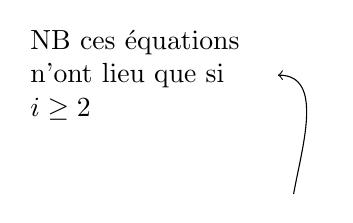
\begin{tikzpicture}
\node[text width=3.1cm,inner sep=1pt] (note) at (0,0) {\uline{NB} ces équations \unsure{n'ont} lieu que si $i\geq2$};
\draw[->] ([xshift=2mm,yshift=-9mm]note.south east) to[out=80,in=0] (note.east);
\end{tikzpicture}}
% The marginal arrow refers to the first line of the preceding brace.

$\sigma_n^2=\mathrm{id}$ tjrs vérifié, $\sigma_n$ est une \uline{réflexion}

Exprimons que $\sigma_0$ est une réflexion.

\[
\deleted{\sigma_0=\left(\begin{array}{ccccc}-1&\lambda_{01}-1&\lambda_{01}-1&\ldots&\unsure{\lambda}\\0&&&&\\\vdots&&&&\\0&&&&\end{array}\right.}
\]
\[
\deleted{\sigma_0(x_1,\ldots,x_{n+1})=\sigma_0(s_0+x_1e_1\ldots+x_{n+1}e_{n+1})}
\]
\[
\deleted{\sigma_0=}
\]
\[
\sigma_0=\left(\begin{array}{cccccc}
-1&\lambda_{0,1}-1&\lambda_{0,1}-1&\ldots&\lambda_{01}-1&1\\
0&\lambda_{0,2}&0&&0&0\\
0&0&\lambda_{02}&&0&0\\
\vdots&\vdots&\vdots&&\vdots&\vdots\\
0&0&0&&\deleted{\unsure{0}}\lambda_{02}&0\\
0&0&0&&\deleted{\unsure{\lambda}}0&1
\end{array}\right)
\]
\[
\underbrace{\hspace{7cm}}_{n+1}
\]
% The underbrace spans the first n+1 columns.
\[
\begin{aligned}
\sigma_0(x_1,\ldots,x_{n+1})&=\deleted{\unsure{(1-x_1,(\lambda_{01}-1)+}}\\
&(1-x_1+(\lambda_{0,1}-1)(x_2+\ldots+x_{n+1}),\lambda_{0,2}x_2,\ldots,\lambda_{0,2}x_{n+1})
\end{aligned}
\]
% archive sheet number: 13
\scanpage{15}
Points fixes:
\[
H_0:\left\{\begin{aligned}(\lambda_{02}-1)x_i&=0\quad\text{si }2\leq i\leq n+1\\2x_1+(1-\lambda_{01})(x_2+\ldots+x_{n+1})&=1\end{aligned}\right.
\]
\deleted{\unsure{Si}} Si $\lambda_{0,2}-1$ inv. ces équations s'écrivent \deleted{$x_i=0\quad2\leq i\leq n+1$}
\[
\left\{\begin{aligned}x_i&=0\qquad2\leq i\leq n+1\\2x_1\deleted{\unsure{+}(1-\lambda_{01})(x_2+\ldots+x_{n+1})}&=1\end{aligned}\right.
\]
donc c'est \unsure{une|un} sous-espace linéaire affine de dim $0$ \deleted{\unsure{unique}} si $2$ inv. \deleted{(car. $\neq2$)}\inserted{\deleted{\unsure{si $k\ne0$|unique et non vide}} (car $\neq2$)}, et c'est vide si $2$ nul dans $k$ \inserted{[\deleted{\unsure{donc pas de}} \unsure{même} en car. $2$, l'hyperplan \unsure{à|:} l'infini\ldots)]} -- donc ce n'est pas un hyperplan. Donc il faut que $\lambda_{02}-1$ soit non inv. \inserted{i.e. nul} sur $\forall$ fibre, donc nilpotent, i.e. $\lambda_{02}=1+\unsure{\nu|v}$, $\nu$ nilpotent. Alors les équations deviennent
\[
\left\{\begin{aligned}\nu x_i&=0\qquad2\leq i\leq n+1\\2x_1+(1-\lambda_{01})(x_2+\ldots+x_{n+1})&=1\end{aligned}\right.
\]
\unsure{que c'est|qui est} un hyperplan sur \uline{chaque fibre}, sauf en \deleted{car} car. $2$ si $\lambda_{0,1}=1$, où c'est vide (mais alors on trouve l'hyperplan \unsure{à|:} l'infini).

\margin{introduire la variable d'homogénéité $\unsure{z|2}$ d'où équation $2x_1+(1-\lambda_{0,1})(x_2\ldots+x_{n+1})=z$}
% slanted

Pour que ce soit un hyperplan, \deleted{il f. et s.} \deleted{\unsure{on} si $2$ inv.} aux pts où la car. est $\neq2$ \deleted{\unsure{et bien}} ou $\lambda_{01}-1$ inv., comme \deleted{l'hyperplan est} $H_0$ contenu dans $H'_0$ d'équation $2x_1+(1-\lambda_{01})(x_2\ldots x_{n+1})=z$, il faut qu'on ait égalité; donc que les équations $\nu x_i=0$ \inserted{$(2\leq i\leq n+1)$ (après $\forall$ chgt. de base\ldots)} soient conséquence de la précédente.

\deleted{Si $2$ inv. ceci} \inserted{\unsure{Ceci exige|Cela exige}} exige \inserted{évidemment} que $\nu=0$.

\deleted{Si $2$ non inv. mais $(1-\lambda_{01})$ inv., alors pour $\uline{n\geq2}$ on trouve ces \unsure{conclusions|conditions}. Le cas $n=1$ doit être traité à part\ldots Si $2$ \uline{\unsure{et|est}} $(1-\lambda_{0,\unsure{1|i}})$}
% archive sheet number: 14
\scanpage{16}
\deleted{non inversibles, \unsure{alors} au pt \unsure{considéré} de $\operatorname{Spec}k$, car $(H'_0)_{\unsure{t|\xi}}$ \unsure{est} $=$ hyperplan \unsure{à|:} l'infini\ldots}

On exigera donc
\[
\lambda_{02}=1
\]
\deleted{\unsure{de}} (ce qui suffit à impliquer $\sigma_0^2=\mathrm{id}$) et on posera
\[
\boxed{\lambda_{01}=1+\alpha_0}
\]
de sorte que $\alpha_0$ est l'invariant modulaire des \unsure{polygônes|polygones} réguliers induits par $\Pi$ dans $f_2$\ldots

\deleted{Exprimons que $\sigma_i$ est une}
\[
\left\{\begin{aligned}
\sigma_{0\deleted{\unsure{0}}}&=\begin{pmatrix}
-1&\alpha_0&\alpha_0&\cdots&\alpha_0&1\\
0&1&0&\cdots&0&0\\
0&0&1&\cdots&0&0\\
\multicolumn{5}{c}{\cdots\quad\cdots\quad\cdots}&\\
0&0&0&\cdots&1&0\\
0&0&0&\cdots&0&1
\end{pmatrix}\\[1em]
\sigma_0(x_1,\ldots,x_{n+1})&=(1-x_1+\alpha_0(x_2+\ldots+x_{n+1}),x_2,\ldots,x_{n+1})\\
H_0:\quad2x_1\deleted{\unsure{+}}\unsure{-|+}\alpha_0(x_2+\ldots+x_{n+1})&=1
\end{aligned}\right.
\]
\uline{Exprimons que} $\sigma_i$ est une \uline{réflexion} $(1\leq i\leq n-1)$.

\deleted{$\unsure{H_i}$}
\diagram{\[
\sigma_i=\left(\begin{array}{ccc}
\begin{array}{rcc}
&\overbrace{\hspace{1.3cm}}^{i-1}&\overbrace{\hspace{1cm}}^{2}\\
i-1\left\{\vphantom{\begin{matrix}1\\\vdots\\1\end{matrix}}\right.&\begin{matrix}1&&\\&\ddots&\\&&1\end{matrix}&0\\
2\left\{\vphantom{\begin{matrix}0\\1\end{matrix}}\right.&0&\begin{pmatrix}0&1\\1&0\end{pmatrix}
\end{array}
&\left.\begin{array}{cccc}
\multicolumn{4}{c}{\overbrace{\hspace{4cm}}^{n-i}}\\
\lambda_{i1}&\lambda_{i1}&\cdots&\lambda_{i1}\\
\unsure{\lambda}&\cdots&\cdots&\cdots\\
\deleted{\unsure{\lambda_{i,i-1}\ldots\lambda_i}}&&&\\
\lambda_{i,i}&\lambda_{i,i}&\cdots&\lambda_{i,i}\\
\lambda_{i,i+1}&\lambda_{i,i+1}&\cdots&\lambda_{i,i+1}
\end{array}\right\}\unsure{i+1}
&\left.\begin{matrix}\vphantom{n-i}\\0\\\vdots\\0\\0\end{matrix}\right\}i+1\\
\begin{array}{rcc}
\deleted{\unsure{2}}n-i\left\{\vphantom{\begin{matrix}0\\\vdots\\0\end{matrix}}\right.&\deleted{\unsure{0}}&0\\
\deleted{\unsure{2}}&&
\end{array}
&\begin{matrix}\lambda_{i,i+2}&0&\cdots&0\\0&\lambda_{i,i+2}&\cdots&0\\\cdots&\cdots&\cdots&\cdots\\0&0&&\lambda_{i,i+2}\end{matrix}
&\left.\begin{matrix}0\\0\\\vdots\\0\end{matrix}\right\}n-i\\
0\quad\cdots\quad0&0\quad\deleted{\unsure{0}}0\quad\cdots\quad0&1
\end{array}\right)
\]}
\[
\begin{aligned}
\sigma_i(x_1,\ldots,x_{n+1})\unsure{=|:}{}&(x_1+\lambda_{i\unsure{1|j}}(x_{i+2}\ldots x_{n+1}),x_2+\lambda_{i2}(x_{i+2}\ldots+x_{n+1}),\ldots,\\
&x_{i-1}+\lambda_{i,i-1}(x_{i+2}\ldots x_{n+1}),x_{i+1}+\lambda_{i,i}(\unsure{x_{i+2}|x_{n+1}}\ldots x_{n+1}),\\
&x_i+\lambda_{i,i+\unsure{1|2}}(x_{i+2}+\ldots+x_{n+1}),\lambda_{i,i+2}x_{i+2},\ldots,\lambda_{i,i+\unsure{2}}x_{n+1})
\end{aligned}
\]
% archive sheet number: 15
